%%%%%%%%%%%%%%%%%%%%%%%%%%%%%%%%%%%%%%%%%%%%%%%%%%%%%%%%%%%%%%%%%%%%%%
% How to use writeLaTeX: 
%
% You edit the source code here on the left, and the preview on the
% right shows you the result within a few seconds.
%
% Bookmark this page and share the URL with your co-authors. They can
% edit at the same time!
%
% You can upload figures, bibliographies, custom classes and
% styles using the files menu.
%
%%%%%%%%%%%%%%%%%%%%%%%%%%%%%%%%%%%%%%%%%%%%%%%%%%%%%%%%%%%%%%%%%%%%%%

\documentclass[12pt]{article}

\usepackage{sbc-template}

\usepackage{graphicx,url}

\usepackage[brazil]{babel}   
\usepackage[utf8]{inputenc}  

     
\sloppy

\title{Detecção de Arritmias Cardíacas com WiSARD}

\author{Ygor Canalli\inst{1}}


\address{
  Programa de Engenharia de Sisemas e Computação\\
  COPPE - Universidade Federal do Rio de Janeiro (COPPE/UFRJ)
  \email{canalli@cos.ufrj.br}
}

\begin{document} 

\maketitle

% \begin{abstract}
%   This meta-paper describes the style to be used in articles and short papers
%   for SBC conferences. For papers in English, you should add just an abstract
%   while for the papers in Portuguese, we also ask for an abstract in
%   Portuguese (``resumo''). In both cases, abstracts should not have more than
%   10 lines and must be in the first page of the paper.
% \end{abstract}
     
\begin{resumo} 
  Este trabalho tem por objetivo avaliar o desempenho do modelo WiSARD no problema de classificar arritmias cardíacas. Utilizando-se da técnica de \emph{bleaching}, uma codificação adequada da entrada, além da criação de classificadores especificos de acordo com o sexo do paciente, foi possível ultrapassar em $0,24\%$ a acurácia publicada anteriormente no \emph{Dataset} em questão.
\end{resumo}


\section{Introdução}

Ao longo dos anos diversas técnicas computacionais tem sido empregadas no problema de dectar e classificar arritmias cardíacas a partir da análise de sinais de Eletrocardiograma (ECG). Podemos destacar técnicas como Projeção de Features~\cite{guvenir1997supervised}, Métodos de Lógica Nebulosa~\cite{salem2009machine, Ijaecs110}, Redes Neurais Artificiais (ANN)~\cite{salem2009machine, Ijaecs110}, Máquinas de Vetores de Suporte (SVM)~\cite{salem2009machine, Ijaecs110}, Modelo Oculto de Markov~\cite{salem2009machine}, Processamento de Sinais~\cite{Ijaecs110} e Computação Evolucionária~\cite{Ijaecs110, martin2014cardiac}.

O objetivo do presente trabalhor é avaliar o desempenho do modelo WiSARD~\cite{aleksander1984wisard} no problema de classificação de arritmias cardíacas. Para tanto, será utilizado o mesmo \emph{Dataset} utilizado em~\cite{guvenir1997supervised}, no qual o modelo supervisionado VFI5, desenvolvido especialmente para o problema, foi capaz de alcançar uma acurácia de $62\%$.

A divisão texto é como segue: no Capítulo~\ref{sec:dados} o \emph{Dataset utilizado é descrito}; o Capítulo~\ref{sec:solucao} descreve como o modelo WiSARD foi utilizado para obter-se bons resultados no problema de classificação de arritmias cardíacas; o Capítulo~\ref{sec:resultados} apresenta os resultados obtidos no presente estudo. Por fim, o Capítulo~\ref{sec:conclusao} traz uma conclusão ao trabalho.

\section{Descrição dos Dados} \label{sec:dados}

O Dataset utilizado foi desenvolvido especialmente para avaliação do Algoritmo VFI5~\cite{guvenir1997supervised}, e foi disponibilizado em~\cite{uci}. O Dataset possui 452 amostras, cada qual relativa a um paciente, e está dividido em 16 classes:
\begin{enumerate}
 \item Normal \label{tipo1}
 \item Mudanças isquemicas (Doença da Artéria Coronária)
 \item Infração Miocardial Anterior
 \item Infração Miocardial Inferior
 \item Taquicardia do Sinus
 \item Braquicardia do Sinus
 \item Contração Centricular Prematura
 \item Contração Supraventriclar Prematura
 \item Bloqueio do Ramo Esquerdo
 \item Bloqueio do Ramo Direito
 \item Bloqueio Atrioventricular de Primeiro Grau \label{tipo11}
 \item Bloqueio Atrioventricular de Segundo Grau \label{tipo12}
 \item Bloqueio Atrioventricular de Terceiro Grau \label{tipo13}
 \item Hipertrofia do Ventrículo Esquerdo
 \item Flibrilação ou Palpitação Atrial
 \item Outros
\end{enumerate}

O \emph{Dataset} é extremamente desbalanceado, sendo mais da metade das amostras da Classe~\ref{tipo1}. Além disso, as classes~\ref{tipo11},~\ref{tipo12}~e~\ref{tipo13} não possuem instâncias. Assim, a Figura~\ref{fig:distribuicao} apresenta a distribuição das amostras. 

\begin{figure}[ht]
\centering
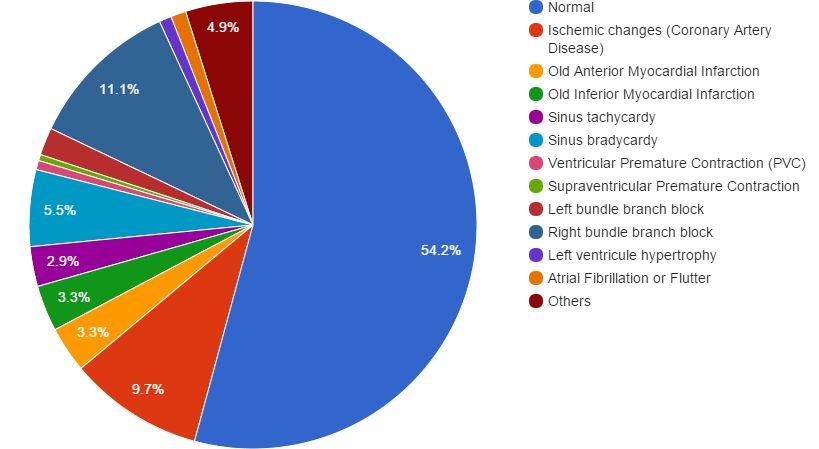
\includegraphics[width=.8\textwidth]{distribuicao.png}
\caption{Distribuição das classes no \emph{Dataset}}
\label{fig:distribuicao}
\end{figure}

Cada amostra é composta por $279$ atributos, dos quais $206$ são contínuos e $73$ categóricos, sendo cerca de $0,43\%$ dos dados contínuos faltosos. Desta forma, parte dos atributos é relativo a informações clínicas, a saber: idade, sexo, peso e altura do paciente; os demais atributos são informações extraídas de ECG. Cada amostra possui informações coletadas a partir de diversos canais do ECG: DI até DIII, V1 até V6, AVR, AVL e AVF. De cada canal são coletadas informações sobre certas ondas especiais, como por exemplo as ondas Q, R e S. A Figura~\ref{fig:ecg} mostra um trecho ilustrativo de ECG apresentando tais ondas. Adicionalmente, são trazidas informações gerais sobre o eletrocargiograma, como por exemplo a frequência cardíaca e valores médios dentre todos os canais. A lista completa de atributos extraidos do ECG é apresentada abaixo.


\begin{itemize}
 \item Informações relativas a cada canal
 \begin{itemize}
  \item Largura média (mseg) das ondas: Q, R, S, R' e S'
  \item Número de deflecções intrínsicas
  \item Existência de imperfeições nas ondas: R, P e T
  \item Existência de derivação difásica nas ondas: R, P e T
  \item Amplitude ($0,1$ * milivolt) das ondas: JJ, Q, R, S, R', S', P e T
  \item QRSA (soma das áreas de todos os segmentos dividido por $10$)
  \item QRSTA (QRSA + $0,5$ * [largura da onda T] * $0,1$ * [altura da onda T])
 \end{itemize}
 \item Informações gerais
 \begin{itemize}
  \item Média das durações (mseg) QRS 
  \item Média dos intervalos (mseg): P-R, Q-T, T-T e P-P
  \item Ângulos do vetor (graus) no plano frontal de: QRS, T, P, QRST e J
  \item Frequência cardíaca (bpm)
 \end{itemize}
\end{itemize}

\begin{figure}[ht]
\centering
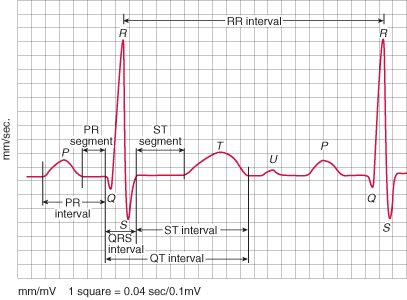
\includegraphics[width=.5\textwidth]{ecg.png}
\caption{Ondas do Eletrocardiograma. Fonte:~\cite{fastlane}}
\label{fig:ecg}
\end{figure}

\section{Detectando Arritmias Cardíacas} \label{sec:solucao}

Utilizando-se do modelo WiSARD convencional, podemos treinar um classificador com os dados do \emph{Dataset} anteriormente discrito, capaz de distinguir dentre os 16 possíveis diagnósticos de arritmia cardíaca. Primeiramente, como existem dados contínuos faltosos, estes foram preenchidos com o valor médio do atributo.
Além disso, como trata-se de um mecanismo capaz apenas de utilizar informações binárias para reconhecimento de padrões, será necessário codificar os dados contínuos e categóricos de maneira adequada, assunto sobre o qual passamos a falar.

Os atributos contínuos foram codificados através da Codificação Termômetro, a qual expressa a magnitude do número através da quantidade de bits $1$ à direita. São divididos $n$ intervalos equidistantes entre os valores mínimos e máximos do atributo, de forma que chamamos $n$ \emph{tamanho do termômetro}. Assim, verifica-se qual o $i$-ésimo intervalo ao qual um certo valor pertence, sendo este representado pela sequência binária de $n$ díditos, na qual os $i$ algarismos à direita são $1$ e os demais $0$. A Tabela~\ref{tab:termometro} apresenta um exemplo de Codificação Termômetro de tamanho $5$, sobre o intervalo de $0$ a $100$.

\begin{table}
\centering
 \begin{tabular}{cc} 
 Intervalo & Codificação termômetro correspondente \\ \hline
 $0\leq x \leq 20$ & $00001$ \\
 $20  < x \leq 40$ & $00011$ \\
 $40  < x \leq 60$ & $00111$ \\
 $60  < x \leq 80$ & $01111$ \\
 $80 < x \leq 100$ & $11111$ \\
 \end{tabular}
  \caption{Exemplo de codificação termômetro de tamanho 5, sobre o intervalo de $0$ a $100$} \label{tab:termometro}
\end{table}

Os atributos categóricos foram representados através de \emph{One-Hot-Encoding}, o qual consiste numa sequência binária com apenas um bit $1$, de forma que a categoria é distinguida pela posição de ocorrência deste bit positivo. A quantidade de bits utilizada na representação é dada pela quantidade de valores distintos que o campo pode assumir. A Tabela~\ref{tab:onehot} ilustra o funcionamento da codificação para um atributo categórico cujos possíveis valores são $A$, $B$, e $C$.

\begin{table}
\centering
 \begin{tabular}{cc} 
 Categoria & \emph{One-Hot-Enconding} correspondente \\ \hline
 $A$ & $001$ \\
 $B$ & $010$ \\
 $C$ & $100$ \\
 \end{tabular}
  \caption{Exemplo de \emph{One-Hot-Enconding} para as categorias $A$, $B$, e $C$} \label{tab:onehot}
\end{table}

Durante a realização dos experimentos, constatou-se que frenquentemente ocorriam empates dentre os descriminadores, fazendo com que o classificador cometesse muitos equívocos. Para contornar a situação, utilizou-se da técnica de desempate Bleaching~\cite{Grieco:2010:PPE:1751674.1751890}, tendo-se estipulado um limite máximo de bleaching arbitrário de valor $15$. Tal limite foi estipulado pois em certos casos o limiar de bleaching subia indefinidamente sem que fosse possível desempatar. O valor $15$, escolhido de maneira arbitrária, pode ser justificado pelo fato de que frequentemente um limiar de valor abaixo de $5$ era suficiente para desempatar, excetuando-se principalmente nos casos no qual o limiar de bleaching subia indefinidamente.

O \emph{Dataset} foi particionado em duas partições, selecionando-se as amostras por sexo, de forma que foi treinado um classificador exclusivo para cada partição. Tal divisão proporcionou uma melhora significativa na acurácia do modelo, se comparado ao treinamento com o \emph{Dataset} por inteiro num único classificador.

Tal organização do modelo proporciona alguns parâmetros que podem ser ajustados, os quais são: o tamanho do termômetro e o tamanho de endereçamento (o qual define a quantidade de RAMs). Além disso, também podemos avaliar qual combinação do uso de parâmetros apresenta melhor acurâcia: apenas categórigos, apenas contínuos ou ambos. Para um ajuste destes parâmetros, utilizamos o método Grid Search, o qual consiste simplemeste na avaliação de todas as combinações possíveis dada uma lista de valores admissíveis para cada parêmtro.

Os tamanhos de termômetro avaliados foram de $4$ a $15$, de forma que a quantidade de colunas da matriz codificada pode variar. Com isso, a lista de valores admissíveis de tamanho de endereçamento foi construída dinâmicamente de acordo com a quantidade de colunas existentes, sendo selecionados os $5$ primeiros divisores não triviais da quantidade de colunas, de forma a se utilizar totalmente o endereçamento de cada uma das RAMs criadas. Por exemplo, para uma matriz codificada que possui $3090$ colunas, avaliamos os tamanhos de endereçamento $2,\,3,\,5,\,6$ e $10$, produzindo respectivamente $1545,\,1030,\,618,\,515$ e $309$ RAMs.

\section{Resultados} \label{sec:resultados}

Os experimentos foram desenvolvidos na linguagem Python, e executados numa máquina com processador Intel(R) Core(TM) i7-4510U CPU @ 2.00GHz e $8$GB RAM, no Sistema Operacional Microsoft(R) Windows 10.

A avaliação da acurácia do classificador deu-se através do $10$-\emph{fold-cross-validation}, na qual o \emph{Dataset} é dividido aleatoriamente em $10$ fatias de mesmo tamanho, avaliando-se o desempenho do classificador em $10$ rodadas. Na $i$-ésima rodada a $i$-ésima fatia é utilizada como conjunto de teste, e as demais como conjunto de treinamento. O processo de treinamento e teste é repetido $10$ vezes, tomando cada uma das fatias como conjunto de teste, e aferindo-se a acurácia média dentre todas as rodadas.

Avaliando-se todas as configurações descritas anteriormente através da técnica $10$-\emph{fold-cross-validation}, a melhor configuração avaliada atingiu a acurácia de $62,24\%$, sendo esta descrita abaixo:

\begin{itemize}
 \item Uso dos atributos: apenas contínuos
 \item Tamanho do termômetro: 14 bits
 \item Tamanho de endereçamento: 4 bits
\end{itemize}

\section{Conclusão}\label{sec:conclusao}

Podemos concluir que o modelo WiSARD foi capaz de atingir resultados de boa qualidade no problema de classificação de arritmias cardíaca, apresentando uma acurácia superior em $0,24\%$ ao resultado publicado para o \emph{Dataset} em questão. Também pode-se perceber que a codificação da entrada é uma etapa crucial para o um bom aproveitamento do modelo. Adicionalmente, o particionamento do \emph{Dataset} de acordo com o sexo foi essencial na obtenção de resultados equiparáveis ao publicado.

\bibliographystyle{sbc}
\bibliography{sbc-template}

\end{document}
